\section{Nouveautés du logiciel}

	L'analyse détaillée d'ADtool a permis de mieux nous rendre compte des fonctionnalités d'analyse qui lui font défaut. Plutôt qu'implémenter ces dernières directement dans ADTool, et risquer ainsi de surcharger % préciser explication.
	ce logiciel, nous avons décidé de créer un nouveau logiciel nommé \glasir qui utilisera un éditeur d'arbres. Nous avons ainsi ADTool qui se chargera de la partie \textit{édition des arbres}, et notre logiciel qui se chargera de la partie \textit{analyse}. Nous avons choisi d'implémenter trois fonctionnalités principales, qui nous semblent répondre le mieux aux besoins d'un expert en sécurité.

		\subsection{Optimiseur}
		\label{subsection:optimiseur} 
		Actuellement, une fois que l'expert a obtenu son arbre complet (qui peut se composer de plusieurs milliers de nœuds), il ne peut pas facilement identifier le chemin optimal (selon un paramètre donné).
		Il s'agit en effet d'un travail manuel, relativement fastidieux, qui doit être recommencé à chaque modification de l'arbre.
		
		Pourtant, la méthode utilisée est systématique. Nous pouvons donc l'automatiser dans notre logiciel. Pouvoir identifier automatiquement le chemin optimal ferait gagner beaucoup de temps à l'utilisateur, et permettrait aussi de limiter les risques d'erreurs.
		
		L'optimiseur prendrait donc en entrée:
		\begin{itemize}
			\item un arbre provenant du projet ;
			\item le paramètre à prendre en compte ;
			\item le critère ($min$ ou $max$).
		\end{itemize}
		
		Nous obtiendrons en sortie un nouvel arbre (qui sera un sous ensemble de l'arbre d'entrée), contenant le chemin optimal. 
		L'utilisateur pourra ensuite le traiter comme un tout nouvel arbre, en fonction de son besoin.
		
		Nous allons maintenant détailler l'algorithme % PK FAIRE ?
		.utilisé. Il s'agira d'une fonction récursive.

		\begin{lstlisting}
opti(racine, param, crit):
	l_fils = fils(racine)

	if vide(l_fils):
		return

	if mode(racine) == ou:
		v = param(l_fils[0])

		for n in l_fils[1:]:
			v = crit(v, param(n))

		for n in l_fils:
			if not defense(n) and param(n) != v:
				delete(n) // will delete subtrees as well
	
	for n in fils(racine):
		opti(n, param, crit)
		\end{lstlisting}

		L'algorithme modifiera l'arbre en l'état (c'est pour cela que nous le ferons travailler sur une copie de l'arbre).
		\begin{itemize}
			\item \verb|racine| correspond au nœud à partir duquel nous élaguerons l'arbre.
			\item \verb|param| est une fonction renvoyant une valeur pour un nœud donné.
			\item \verb|crit| est une fonction prenant en paramètre deux valeurs et renvoie la valeur à \og garder \fg.
			\item \verb|fils| est une fonction renvoyant une liste de nœuds, correspondants aux fils du nœud passé en paramètre.
		\end{itemize}
		Ainsi, pour lancer l'optimisation, nous appellerons \verb|opti| avec la racine de l'arbre en paramètre.

		Prenons en exemple l'arbre exemple en Annexe. % ref Annexe
		Si on veut trouver un chemin optimal, avec en paramètre le coût, et en critère la fonction $min$, on obtiendra l'arbre de la figure \ref{fig:arbre_post_opti}.

		\begin{figure}[h!]
			\centering
			\includegraphics[width=0.35\textwidth]{figure/post_optimiseur.pdf}
			\caption{L'attaque optimale est ainsi facilement lisible.}
			\label{fig:arbre_post_opti}
		\end{figure}


	\subsection{Filtre}
	\label{subsection:filtre} 
	
		ADTool met à disposition de l'utilisateur un certain nombre d'outils pour l'assister dans la modélisation de son système, parmi lesquels se trouve la possibilité d'appliquer plusieurs valuations aux nœuds de l'arbre. On peut ainsi pour le même arbre créer une valuation sur la probabilité de l'attaque et une autre sur son coût.

		Souvent, l'utilisateur va chercher à se défendre contre un attaquant précis. Dans ces cas, il va chercher à identifier les ressources dont l'attaquant dispose (temps, argent, personnel humain, etc), ce qui peut l'amener à ne vouloir conserver que les chemins de l'arbre empruntables par l'attaquant en accord avec ses ressources. Dans ce cas, nous comparerons les ressources de l'attaquant avec les valuations de l'arbre.

		En l'état, ADTool ne permet pas de faire cette sélection. Nous allons donc implémenter cette fonctionnalité dans notre logiciel, sous le nom de \textit{filtre}. % l'objectif sera de comparer...

		La fonction de filtrage prendra en entrée : 
		\begin{itemize}
			\item L'arbre à filtrer ;
			\item Les valuations de l'arbre servant de critères pour le filtrage ;
			\item Les intervalles de sélection sur les différentes valuations.
		\end{itemize} % pas assez en évidence ? 

		Le filtre proposera deux types d'intervalles à l'expert pour chacune des valuations :
		\begin{itemize}
			\item L'intervalle global, qui devra être respecté par chacun des chemins conservés, dans le sens où la valuation du chemin dans son ensemble rentre dans l'intervalle ;
			\item L'intervalle unitaire, qui devra être respecté par la valuation de chacun des nœuds pour les chemins retenus.
		\end{itemize} % REFORMULER

		Il est possible de filtrer l'arbre avec plusieurs paramètres simultanément.
		L'arbre retourné par la fonction de filtrage sera l'arbre d'origine élagué. Seuls seront conservés les chemins respectant les intervalles de filtrage.
		
		Par exemple, en appliquant un filtre global [0, 500] sur le coût à l'arbre exemple en Annexe, on obtient l'arbre de la figure \ref{fig:arbre_post_filtre}.

		\begin{figure}[h!]
			\begin{center}
				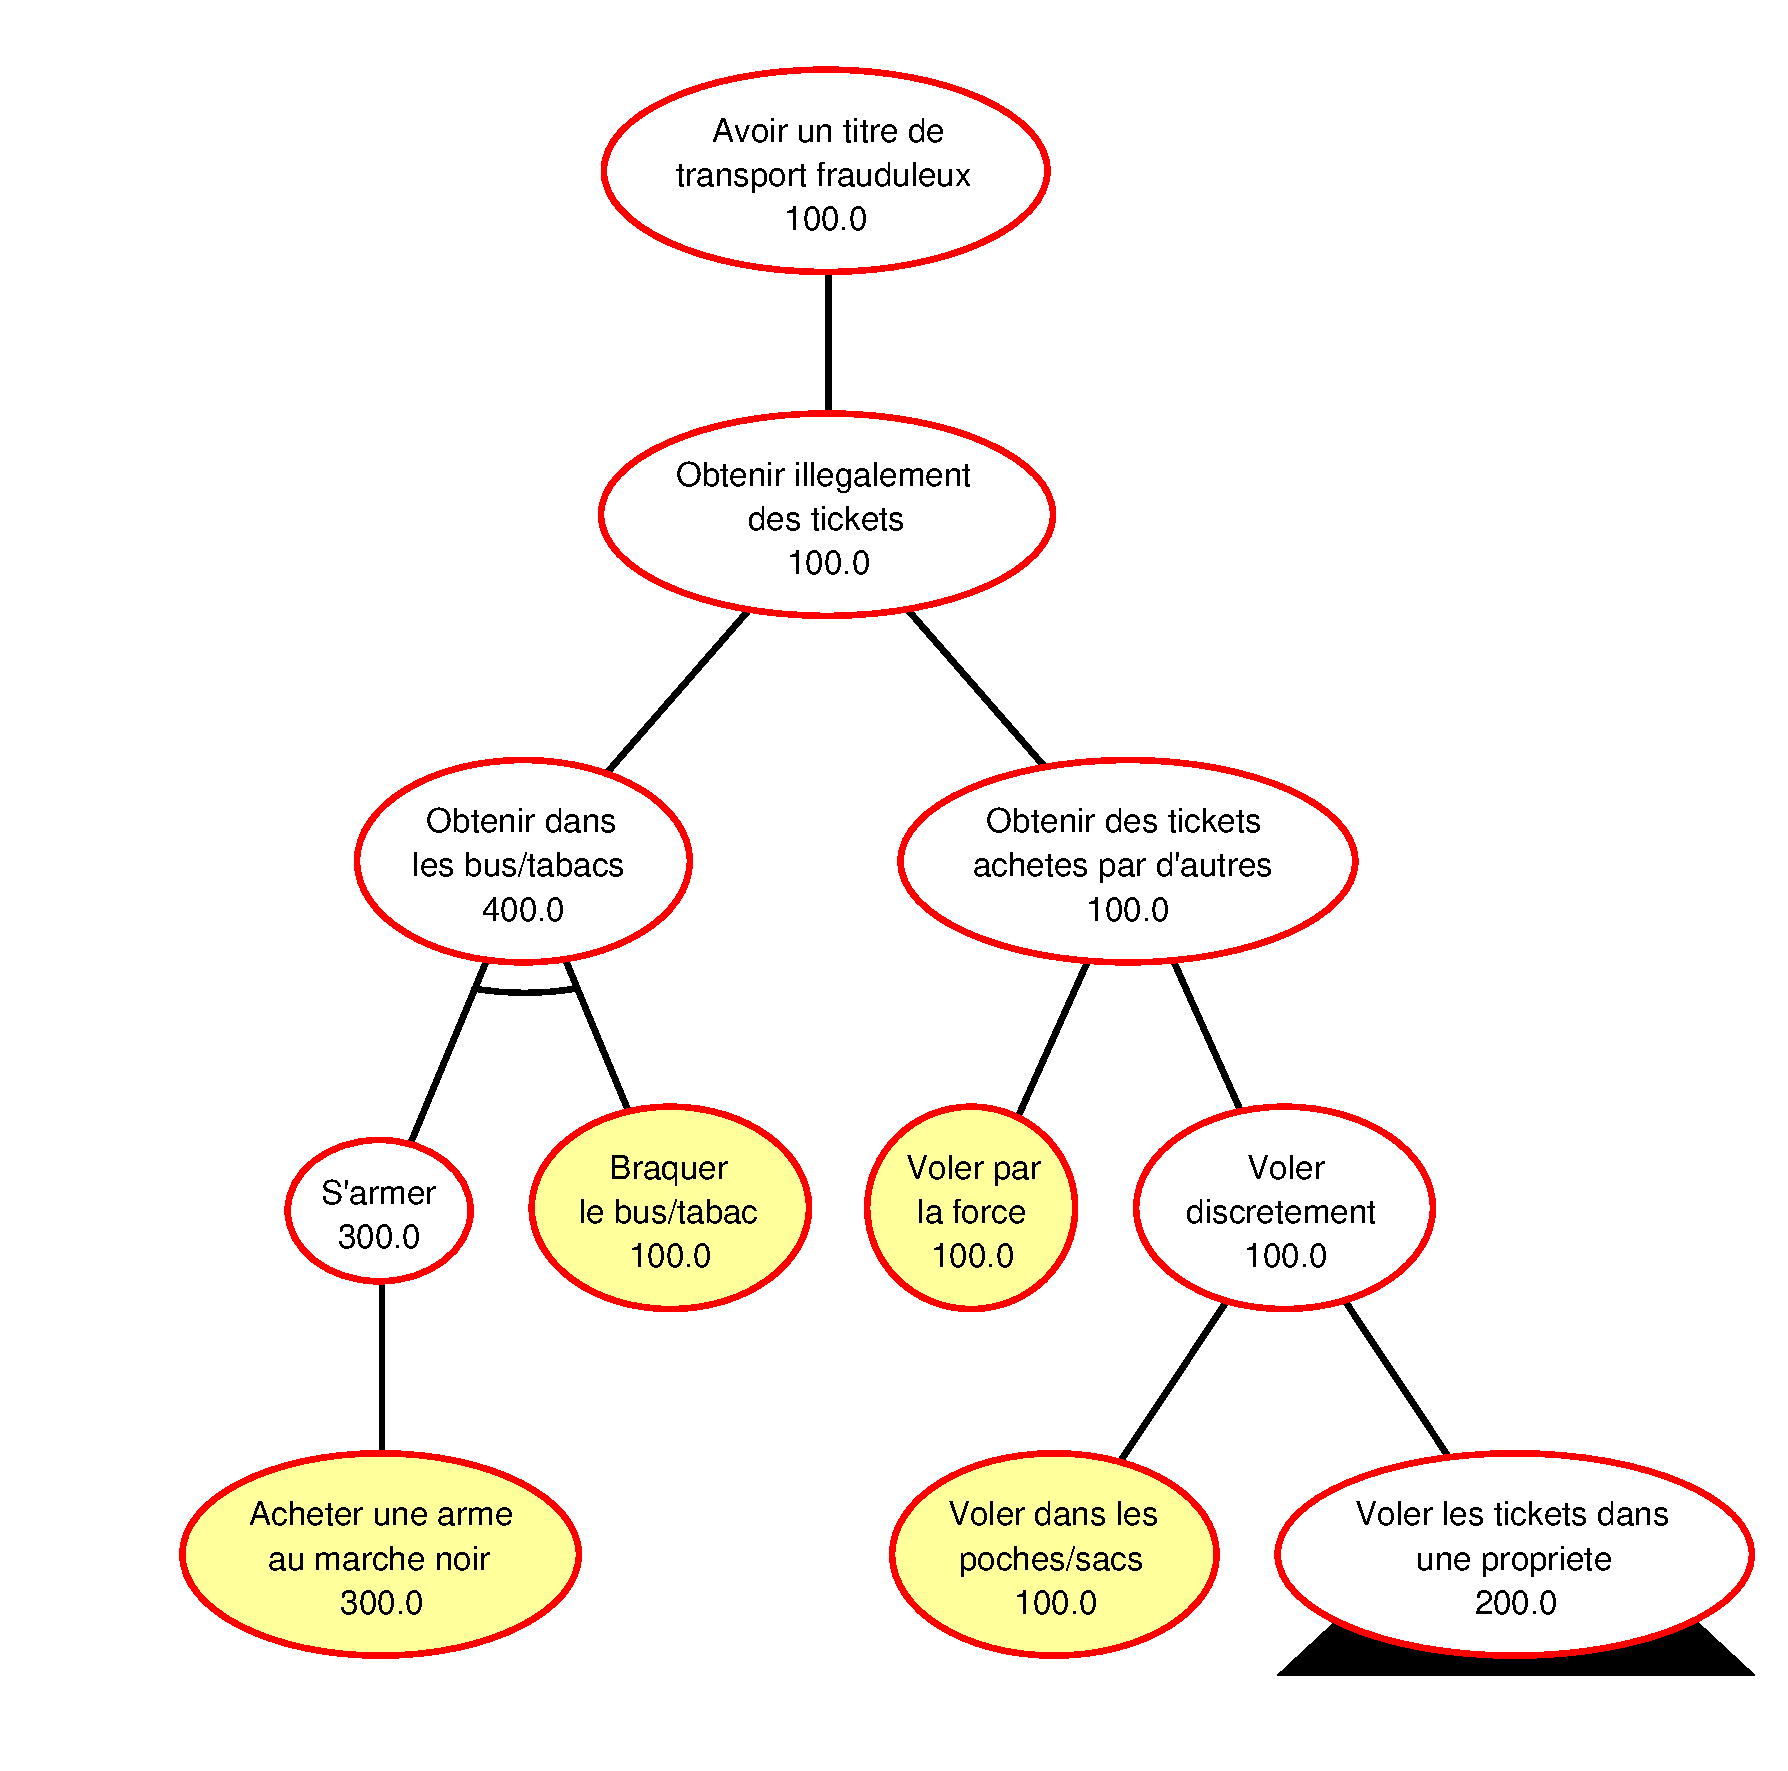
\includegraphics[width=0.75\textwidth]{figure/post_filtre.pdf}
			\end{center}
			\caption{Filtre selon le coût pour l'attaquant}
			\label{fig:arbre_post_filtre}
		\end{figure}

		On constate que l'arbre élagué par le filtre est beaucoup plus concit. En ayant en tête que l'arbre exemple est de taille très réduite comparée aux modélisations de systèmes réels, on comprend bien l'utilité de cette fonctionnalité pour l'expert.   

		D'un point de vue technique, il nous semble intéressant de quelle manière l'arbre sera élagué par le filtre.
		L'algorithme de filtrage suivra ce modèle :

		\begin{lstlisting}

filtre(racine, rules) :
	for r in rules :
		if not r(racine) :
			delete (racine AND subtrees)
			return

	for n in fils(racine) :
		filtre(n, rules)

		\end{lstlisting}
	
		Le principe de l'algorithme est récursif.
		Le nombre d'appel récursif sera, au pire, linéaire avec le nombre de nœud de l'arbre.
		La complexité algorithmique est donc acceptable.

		\subsection{Paramètres de synthèse}
		\label{subsection:synthese} 

			L'utilisateur est actuellement cantonné aux paramètres présentés précédemment dans la section 2, et ne peut pas en créer d'autres, ce qui limite ses possibilités d'analyse et d'interprétation. En effet, les paramètres déjà existants ne sont pas les seuls pouvant intéresser un expert en sécurité. Nous souhaitons donc rendre possible la création de nouveaux paramètres, à partir de ceux déjà disponibles et des fonctions mathématiques de base (division, multiplication, min, max, etc). Ces nouvelles valuations pourront ensuite être appliquées à n'importe quel arbre, de la même manière que les paramètres de base. Elles pourront ainsi être utilisées pour analyser les arbres selon de nouveaux critères, et si besoin pour les élaguer à l'aide du filtre que nous allons implémenter.\\

			Cette nouvelle fonctionnalité, appelée \emph{éditeur de paramètres}, prendrait donc en entrée les éléments suivants :
			\begin{itemize}
				\item un arbre provenant du projet courant; % quel projet ?
				\item les paramètres intervenant dans la synthèse ;
				\item les opérations mathématiques appliquées ;
				\item le nom du paramètre de synthèse généré.
			\end{itemize}

			Par exemple, dans notre arbre illustratif disponible en Annexe de ce rapport, nous pouvons voir que les deux sous-arbres « Obtenir illégalement des tickets » (sous-arbre A) et « Falsifier des tickets » (sous-arbre B) permettent d'atteindre l'objectif final. Il est actuellement possible de les valuer par treize paramètres, nous n'en garderons ici que deux pour simplifier : le coût minimal et la probabilité de succès.\\ % figure ?

			On constate rapidement que choisir A implique un coût de réalisation moindre pour l'attaquant puisqu'il nécessite peu de matériel. Cependant, un vol est toujours risqué, et les chances de se faire arrêter sont élevées. Opter pour le sous-arbre B, bien que plus cher à réaliser, permet de limiter ces risques : la probabilité de succès est donc plus forte. On voit donc que ces deux paramètres, qui ne sont pas liés, peuvent être tous les deux utiles à l'utilisateur et entraîner une interprétation très différente. C'est pourquoi il serait intéressant de pouvoir les combiner, grâce à notre éditeur de paramètres, afin de les prendre en compte tous les deux. C'est ensuite à l'utilisateur de juger des liens qu'il désire instaurer entre les paramètres : fonctions mathématiques, coefficients, etc. Par exemple, si l'on décide d'appeler le nouveau paramètre « result », et que l'on estime qu'il s'agit du coût auquel on ajoute la probabilité de succès multipliée par deux, on obtient la synthèse suivante : \[ result = (minimal\_cost) + 2 \times (probability\_of\_success).\]
